\chapter{法律類}
\section{2016年2月15日 (Instructor: Vivian)}
\subsection{無證駕駛}
\subsubsection*{需要掌握的單詞短語}
\begin{itemize}
  \itemsep0em
  \item 疏忽駕駛 / 應照管的責任: driving without \hilight{due care} / duty of care
  \item 罰單 / 罰款: speeding \hilight{ticket} / penalty notice
  \begin{center}
    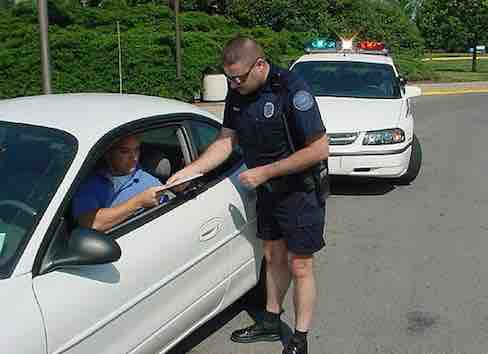
\includegraphics[scale=.5]{pics/speeding-ticket.jpg}
  \end{center}
  \item 駕駛執照: driver’s licence
  \item 臨時吊銷駕照 / 徹底吊銷駕照: \hilight{suspend} the licence / \hilight{revoke} the licence
  \item 疲勞駕駛 (的行為): fatigue driving 也可以譯作 \hilight{drowsy} driving / driving tired
  \item 超載: overload
  \item 罪犯, 違法 / 違章 / 違規者: offender (offence指違法行為)
  \item 違章: Road \& Traffic Offence
  \item PCA\footnote{詳情參考: \url{http://adamslawyers.com.au/prescribed-concentration-of-alcohol-and-drink-driving/}} : Prescribe Concentration of Alcohol (規定的酒精濃度)
  \item BAC: Blood Alcohol Content / Concentration (血液酒精濃度)
  \item RBT: Random Breath Test (隨機呼吸酒駕測試)
  \item (除酒外的)飲料: soft drinks / alcohol-free drinks
  \item 嚴重性: seriousness
  \item 委婉地謝絕(喝酒): decline (不用refuse或reject)
  \item 靠邊停車 / 把車開走: \hilight{pull over}  / pull out (也可以指突然發動車子)
  \begin{center}
    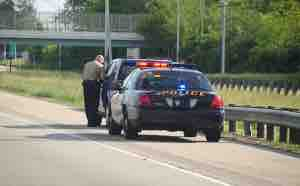
\includegraphics[scale=.7]{pics/pull-over}
  \end{center}
  \item 報名參加考試: register for the exam test
\end{itemize}

\subsubsection*{需要掌握的句型}
\begin{itemize}
  \itemsep0em
  \item She just arrived here / in Australia not long ago = She hasn’t been here very long.
  \item 我是一個奉公守法的人: I am a \hilight{law-abiding} person.
  \item 勸服: persuade sb. to do sth.
  \item 勸我喝酒: make me drink (urge sb. to do sth.)
  \item 我哪裡做錯了: Have I done anything wrong? / What have I done wrong?
  \item 把某人攔到一邊: \hilight{pull sb. over}
  \item 壓線行駛: straddle the \hilight{edge} of the lane
  \item 我知道是為什麼了: I see that’s why.
\end{itemize}

\subsection{跨道駕駛}
\subsubsection*{需要掌握的單詞短語}
\begin{itemize}
  \itemsep0em
  \item RTA: Road \& Traffic Authority 道路交通管理局\footnote{現在已經被合併到了Services NSW}
  \item 公路\hilight{海事}管理局: Road \& \hilight{Maritime} Service
  \begin{center}
    
\includegraphics[scale=.5]{pics/rms}
  \end{center}
  \item 正常的公路(非高速公路): highway
  \item 高速公路: freeway / express way / motorway
  \item 單子(一般指罰單): ticket / notice (但一般不說slip)
  \item 學習駕照: learner’s licence
  \item 全牌駕照 / 正式駕照: full licence
\end{itemize}

\subsubsection*{需要掌握的句型}
\begin{multicols}{2}
\begin{itemize}
  \itemsep0em
  \item Enquire about = make enquires about sth.
  \item 瞭解情況: get some information about…
  \item \hilight{當事人}都有誰: Who was involved?
  \item 事情的詳細經過是什麼: What happened exactly?
  \item 謝謝你能安排時間過來: Thank you for taking time to come.
  \item 我當時持有L牌: I was holding a learner’s licence.
  \item 我的駕駛技術不熟練: I am not a skilled driver.
  \item 在左右車道上: \hilight{in} the left / right lane
\end{itemize}
\end{multicols}

\subsubsection*{注意}
\begin{itemize}
  \itemsep0em
  \item 表達時間+日期:
  \begin{itemize}
    \itemsep0em
    \item It was at 8.30 in the morning, and on 30th of June.
    \item It was at 8.30 AM / PM \hilight{of} the 30th of June.
  \end{itemize}
  \item 當指``一個警察"的時候, 不要光說police, 要說\hilight{police officer}.
\end{itemize}

\subsection{家長會 (2015年12月11日真題)}
\subsubsection*{需要掌握的單詞短語}
\begin{multicols}{2}
\begin{itemize}
  \itemsep0em
  \item (在學校的)成績: academic performance
  \item 聽話: well behave
  \item \hilight{懂禮貌}, 尊敬別人的: respectful
  \item (課堂上)跟得上: catch up / keep up in class
  \item 鑒於 / 考慮到: given the fact…
  \item 家庭讀物: home reader
  \item 補習班: cram school (少用) / \hilight{coaching class} / tutoring class / coaching session
  \item (課上)認真聽講: concentrate in class
\end{itemize}
\end{multicols}

\subsubsection*{需要掌握的句型}
\begin{multicols}{2}
\begin{itemize}
  \itemsep0em
  \item 她聽話嗎: Has she be well-behaved?
  \item 在某方面幫助某人: help sb. with sth.
\end{itemize}
\end{multicols}

\subsubsection*{注意}
\begin{itemize}
  \itemsep0em
  \item Whether起頭的句子不是疑問句,  因此後面接的句子必須是陳述句語序.
\end{itemize}

\subsection{糖尿病 (2015年12月11日真題)}
\subsubsection*{需要掌握的單詞短語}
\begin{itemize}
  \itemsep0em
  \item (測量的)指標, 結果: reading
  \item 惡化: \hilight{deteriorate} / worsen
\end{itemize}

\subsubsection*{需要掌握的句型}
\begin{itemize}
  \itemsep0em
  \item 以防我忘記: in case I forget
  \item 最近視力模糊: my vision has been blurred recently
  \item 活不下去了: life is so hard
\end{itemize}

\subsubsection*{注意}
\begin{itemize}
  \itemsep0em
  \item 目前學過的虛擬語氣有兩種: I wish I had… 和 Should have done…
  \item \hilight{Since + 過去時 翻譯成``自從", Since + 完成時 翻譯成``因為"}
\end{itemize}

\subsection{法律咨詢(樓上夫妻吵架)}
\subsubsection*{需要掌握的單詞短語}
\begin{itemize}
  \itemsep0em
  \item 回想下: take back to (接時間 / 日期)
  \item 住在我們樓上 / 樓下的: live above / under us
  \item 吵架: argue
\end{itemize}

\subsubsection*{需要掌握的句型}
\begin{itemize}
  \itemsep0em
  \item 可能會出人命: someone's life might be in danger
  \item 無能為力: We couldn't help much.
\end{itemize}

\subsection{酒後駕車}
\subsubsection*{需要掌握的單詞短語}
\begin{multicols}{2}
\begin{itemize}
  \itemsep0em
  \item 聽證, 庭審: trail / court \hilight{hearing}
  \item \hilight{公訴人 / 公訴: prosecutor / prosecution}
  \item 減輕對我的處罰: reduce my punishment / impose a lenient penalty on me
  \item 網開一面 / 寬容: be lenient ($adj.$)
  \item 法官大人(稱呼): Your honour
  \item 巡邏警察: police on patrol
  \item (他們)老實點: behave themselves
  \item 酒醒了: \hilight{sober} ($adj.$)
  \item 一杯酒 / 牛奶: one glass of beer / milk
  \item 正當的 / 充分的理由: good reason
  \item 法庭的判決: court decision
  \item 付款 / 付清: pay / pay off
  \item \hilight{初犯: first time offender}
\end{itemize}
\end{multicols}

\subsubsection*{需要掌握的句型}
\begin{multicols}{2}
\begin{itemize}
  \itemsep0em
  \item 我(不)認罪: I plead (not) guilty.
  \item 用良好行為擔保: put $sb.$ on the good behaviour bond.
  \item 考慮: take $sth.$ into account / consideration
  \item 判你死刑: sentence you to death
  \item 我不是故意不配合: I didn't means to be uncooperative
  \item (方位)在我前面的人: the person in front of me
  \item 大大地影響收入: affect income greatly
  \item 真心的悔改: sincerely repentant
  \item 放我走: let me off
\end{itemize}
\end{multicols}

\subsection{駕駛執照 (第一部分)}
\subsubsection*{需要掌握的單詞短語}
\begin{itemize}
  \itemsep0em
  \item 分階段駕照制度: Graduated Licensing Scheme (Graduated 千萬不要翻譯成畢業生!)
  \item 臨時駕照: provisional licence (包括 Phase I / II (第一 / 第二階段))
  \item plate $\xrightarrow{\text{的人}}$ plater (翻譯成持有人, 等同於holder)
  \item 適合某人: suit someone's need
  \item 個人的需求: individual personal needs
  \item 和考駕照考試有關的詞:
  \begin{itemize}
  \itemsep0em
    \item 路況知識: knowledge about road
    \item \hilight{危險意識}測試: \hilight{Hazard Perception} Test
    \begin{center}
      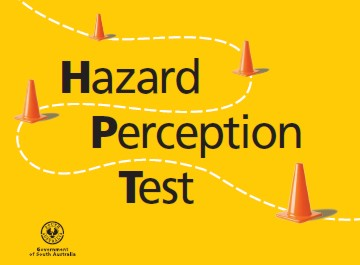
\includegraphics[scale=.5]{pics/hpt}
    \end{center}
    \item 駕駛員資格測試: Driver Qualification Test
    \item 機動車登記處: Motor Register
    \item 駕駛員知識測試: Driver Knowledge Test
  \end{itemize}
\end{itemize}

\subsubsection*{需要掌握的句型}
\begin{itemize}
  \itemsep0em
  \item 剛滿16週歲: just turned 16
  \item 這是我最大的顧慮: This is my biggest concern.
  \item \hilight{佔(比例): take up / account for}
  \item 從...過渡到: progress from ... to ...
  \item 一個較長的時間里: an extended period of time / over a period of time
  \item 同意某事: \hilight{be in favor of $sth.$}
  \item 把這個信息轉告他: \hilight{pass on} this information to him.
\end{itemize}

\subsection{駕駛執照 (第二部分)}
\subsubsection*{需要掌握的單詞短語}
\begin{multicols}{2}
\begin{itemize}
  \itemsep0em
  \item 交通法規 / 道路規章: road rule
  \item L牌(泛指): Ls
  \item clever (一般指小齡兒童) $\xrightarrow{\text{的人}}$ smart (指大一些的人)
  \item 方便, 好用: \hilight{handy} (This is an OZ expression)
  \item 規定的路線: set course
\end{itemize}
\end{multicols}

\subsubsection*{需要掌握的句型}
\begin{itemize}
  \itemsep0em
  \item 一次考過: pass the test \hilight{on the first try / in one go}
  \item L牌的有效期有多長?: How long is the learner's license valid for?
  \item 對他人的警覺: awareness of other
\end{itemize}

\vspace{15mm}

\begin{center}
  \textbf{************ END OF THE DAY ************}
\end{center}
\newpage

\section{2016年2月16日 (Instructor: Chris)}
\subsection{家庭暴力}
\mybox{\centering \textbf{注意}: 更多筆記被歸納到專題里的``澳洲不同的法院"和``各種打人的方式", 請參考目錄查找!}
\subsubsection*{需要掌握的單詞短語}
\begin{itemize}
  \itemsep0em
  \item 普外科\footnote{是以手術為主要方法治療肝臟, 膽道, 胰腺, 胃腸, 肛腸, 血管疾病, 甲狀腺和乳房的腫瘤及外傷等其它疾病的臨床學科}: general surgeon
  \item 流動測醉警車: booze bus
  \begin{center}
      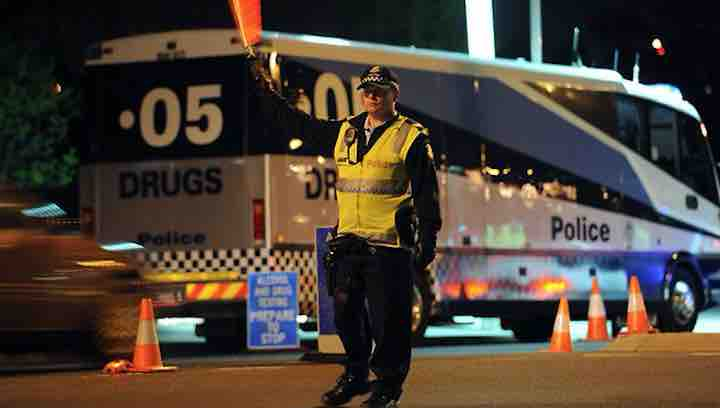
\includegraphics[scale=.5]{pics/booze-bus}
  \end{center}
  \item 酒駕整治行動: booze bus operation
  \item \hilight{Apprehended Violence Order (AVO): 暴力禁止令}
  \item Apprehended Domestic Violence Order (ADVO): 家庭暴力禁止令\footnote{適用於親戚, 同居關係甚至普通室友的關係}
  \item Apprehended Personal Order (APO): 個人禁止令
  \item 恐嚇 / 接近 / 跟蹤: intimidation / approach / stalk
  \item (高級)警員 / 警長(沙展) / 督查 / 警司: \hilight{(senior) constable} / sergeant / inspector / superintendent
  \item (警)問話, 筆錄: interview
  \item \hilight{嘮叨: nag (at)}\footnote{加不加at都可以}
  \item 奚落, 損, 嘲笑: taunt
  \item 打臉: hit \hilight{in} the face
  \item 鼻血: bleeding nose
  \item 頭暈 / 眩暈 / 偏頭痛 / 頭疼: dizziness / vertigo / migraine / headache
  \item 擋一下: block / \hilight{ward it off}
  \item 米蘭達規則: Miranda's Right\footnote{詳情請看 \url{https://www.legalzoom.com/articles/know-your-rights-what-are-miranda-rights}}
  \item 告誡卡\footnote{警察逮捕人時以防罪犯不懂英語, 將米蘭達告誡中文版印在卡上給罪犯看}: caution card
\end{itemize}

\subsubsection*{需要掌握的句型}
\begin{itemize}
  \itemsep0em
  \item 我們現在在說的這個問題: Now we are at it.
  \item \hilight{家醜不可外揚: We don't air the dirty laundry to the public.}
  \item 答到點子上了: answer to the point
  \item 煩死, 受夠某人: be sick (tired) of / be fed up with...
  \item 看不起: look down upon
  \item 你說我怎麼辦?!: You TELL ME what I should do.
  \item 有沒有搞錯?: Are you kidding me? / \hilight{Hello???} (注意語氣)
  \item 她怎麼打我的臉, 我就怎麼打回去: I hit her \hilight{the way} (way 可替換成 like how) she hit me in the face.
  \item 我真沒使這麼大力氣打她: I didn't hit her that hard.
\end{itemize}

\subsection{海關查獲 (第一部分)}
\subsubsection*{需要掌握的單詞短語}
\begin{multicols}{2}
\begin{itemize}
  \itemsep0em
  \item 犯法: breach (break) the law / do $sth.$ illegal / commit offence
  \item 出入境卡: Incoming Passenger Card / Outgoing Passenger Card
  \item 違禁物品: prohibited substances
  \item 行蹤, 下落(代替where): whereabout(s)
  \item 表姐: cousin
  \item 無意中聽到 / 偷聽: overhear / eavesdrop
  \item 欺負, 挑刺: bully / pick on...
  \item 檢疫(犬): \hilight{quarantine} (dog)
  \item 緝毒犬: sniffer dog
  \begin{center}
      
\includegraphics[scale=.3]{pics/sniffer-dog}
  \end{center}
  \item 家禽: poultry
  \item 植物成分: plant material
\end{itemize}
\end{multicols}

\subsubsection*{需要掌握的句型}
\begin{itemize}
  \itemsep0em
  \item 告誡某人: \hilight{caution $sb.$}
  \item 一定很擔心我: must be very worried about me.
  \item 如果你沒有家人在身邊: If you have no family around / by your side
\end{itemize}

\subsection{海關查獲 (第二部分)}
\mybox{\centering \textbf{注意}: 更多筆記被歸納到專題里的``各種法律懲罰", 請參考目錄查找!}
\subsubsection*{需要掌握的單詞短語}
\begin{itemize}
  \itemsep0em
  \item 重新開始, 繼續: resume
  \item \hilight{借進 / 借出: lend / borrow}
  \item (法律上的)說法: story (不要翻譯成故事)
\end{itemize}

\subsubsection*{需要掌握的句型}
\begin{itemize}
  \itemsep0em
  \item 越不想什麼, 越來什麼: The things I have got is what I need the least.
  \item 這是我最不想見到的: The thing I got is the last thing I want.
  \item 陷害某人: set $sb.$ up / frame $sb.$
\end{itemize}

\subsubsection*{其他}
\begin{itemize}
  \itemsep0em
  \item 米蘭達告誡: You have the right to remain silent. Anything you say can and will be used against you in a court of law. You have the right to talk to a lawyer and have him present while you are questioned. If you cannot afford to hire a lawyer, one will be appointed to represent you before questioning, if you wish one.
  \item 米蘭達告誡譯文: 你有權保持沈默,否則你所說的一切,都能夠、而且將會在法庭上作為指控你的不利證據;\\ 審問之前,你有權與律師談話,得到律師的幫助和建議;你受審問時你有權讓律師在場;\\ 如果你想聘請律師但卻負擔不起,法庭將為你指定一位律師.
\end{itemize}

\subsection{工傷賠償}
\subsubsection*{需要掌握的單詞短語}
\begin{multicols}{2}
\begin{itemize}
  \itemsep0em
  \item 工傷賠償: worker's comp / compo
  \item \hilight{工傷: worker-related injury}
  \item 工傷保險: Work Cover
  \item (全身)升降機: (full) body lifter
  \item \hilight{腰間盤突出: slipped disk(s)}
  \item 腰 / 腰圍: (lower) back / wrist
  \item 腦中風: stroke
  \item 中風病人: A stoke patient
  \item 上級的(護士): supervising nurse\footnote{大多數時候``上級"直接翻譯成supervisor即可.}
  \item 請假: take a leave / apply for a leave
  \item 用腰過度: \hilight{lumber muscle overstrain}\footnote{``曲線救國"的說法: overuse of lower back}
  \item 腰椎: lumbar vertebra (lumbar即是腰的形容詞)
  \item \hilight{康復: rehabilitation}
  \item 戒毒所: Rehabilitation Centre (簡稱\hilight{rehab})
  \item sort out = work out (整理)
  \item 肌肉勞損: Repetitive Strain Injury (RSI)
  \item 鏟車 / 叉車 / 堆高機: forklift
  \begin{center}
      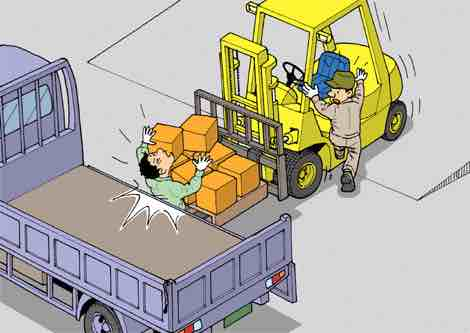
\includegraphics[scale=.3]{pics/forklift}
  \end{center}
  \item 裝貨 / 卸貨: load (unload)
  \item \hilight{倒車: reverse}
  \item 粉碎性骨折: \hilight{comminuted fracture}
  \item 間歇的: intermittent
\end{itemize}
\end{multicols}

\subsubsection*{需要掌握的句型}
\begin{itemize}
  \itemsep0em
  \item 在去年12月的中旬: in the mid of \hilight{last} December.
  \item 從...掉下來: fall \hilight{off from}...
  \item 劇烈的刺痛: sharp stabbing pain
\end{itemize}

\subsubsection*{注意}
\begin{itemize}
  \itemsep0em
  \item \hilight{請注意``months"的發音!!!}
  \item 不需要一直陪同的``送走"一般用send, 比如救護車把人送走, 但如果是朋友陪同去醫院, 一般用\hilight{``take $sb.$ to the hospital"}
  \item college 可與 workmate 互換
\end{itemize}

\subsection{侵犯隱私}
\subsubsection*{需要掌握的單詞短語}
\begin{multicols}{2}
\begin{itemize}
  \itemsep0em
  \item 惡意的: \hilight{malicious} / evil
  \item 理解: appreciate (這篇文章不翻譯成欣賞)
  \item 對律師的稱呼: Mr. / Ms. Solicitor
  \item 令人不安的: disturbing
  \item \hilight{晾衣服: air the laundry}
  \item 在二樓: on the second floor
  \item 灰色地帶: grey area
  \item 精神病患者, 變態: \hilight{psychopath}, phycho
  \item 色狼: pervert
  \item 確定: establish (這篇文章不翻譯成建立)
  \item 構成(犯罪): constitute
  \item 非法進入: trespass ($v.$ + $n.$)
\end{itemize}
\end{multicols}

\subsubsection*{需要掌握的句型}
\begin{multicols}{2}
\begin{itemize}
  \itemsep0em
  \item \hilight{好像: as if}
  \item 做不了什麼: do very little to...
  \item 我不敢: I don't dare
  \item 侵犯隱私: invasion / violation of privacy
  \item 讓陽光進來: let sunshine / daylight in
  \item 一樣 / 不亞於: no less than
  \item 告他賠錢: sue him for money
  \item (正)對準: point (directly) at...
  \item 而不是...: as oppose to...
  \item 在...的範圍內: within the bound of...
  \item 持續了一陣: over a substantiated period.
\end{itemize}
\end{multicols}

\vspace{15mm}

\begin{center}
  \textbf{************ END OF THE DAY ************}
\end{center}
\newpage

\section{2016年2月22日 (Instructor: Vivian)}
\subsection{遺囑}
\mybox{\centering \textbf{注意}: 更多內容請見法律詞彙專題里的和立遗嘱有关的词汇!}
\subsubsection*{需要掌握的單詞短語}
\begin{multicols}{3}
\begin{itemize}
  \itemsep0em
  \item 報刊亭: news agency
  \item 修改, 修訂: amend ($v.$)
  \item 修正案: amendment ($n.$)
  \item 生孩子(重過程): give birth
  \item 指派, 委派: appoint / nominate
\end{itemize}
\end{multicols}

\subsubsection*{需要掌握的句型}
\begin{multicols}{2}
\begin{itemize}
  \itemsep0em
  \item 我不想鬧上法庭: I don't want to \hilight{end up in} court.
  \item 她剛生了小孩: She has just had baby.
  \item 遺產的比例: \hilight{share} of the estate
  \item 爭奪遺產: fight \hilight{over} estate.
  \item 強烈不建議:
  \begin{itemize}
    \itemsep0em
    \item strongly advise against doing sth.
    \item advise $sb.$ not to do.
\end{itemize}
  \item 關於: as to... / regarding...
  \item 按照你說的做: follow your \hilight{instructions}
\end{itemize}
\end{multicols}

\subsection{永久授權書}
\subsubsection*{需要掌握的單詞短語}
\begin{multicols}{2}
\begin{itemize}
  \itemsep0em
  \item 永久授權書: \hilight{enduring} power of attorney
  \item 代理人, 委託人: agent / attorney
  \item 授權人: principal / grantor / authoriser
  \item 起草: draft / draw up / prepare
\end{itemize}
\end{multicols}

\subsubsection*{需要掌握的句型}
\begin{multicols}{2}
\begin{itemize}
  \itemsep0em
  \item 這是怎麼弄的呢: How can it be done?
  \item 代理我行事: appoint $sb.$ to act on my behalf
  \item 管理: control \hilight{over} $sth.$
  \item 生效: come into effect / become effective / take effect
  \item 法律生效: come into force
  \item 弄完: have $sth.$ done / ready
\end{itemize}
\end{multicols}

\subsection{離婚事宜}
\subsubsection*{需要掌握的單詞短語}
\begin{multicols}{2}
\begin{itemize}
  \itemsep0em
  \item 孩子撫養權: child custody
  \item 孩子撫養費: child support (或maintenance)
  \item 配偶撫養費: alimony
  \item 監護權(不一定指離婚後): guardianship
  \item 孩子的探視權: access to child
  \item 撫養令 / 安排: parenting order / arrangement
  \item 復合, 重歸於好: get back together / reconciliation
  \item 提出離婚申請: lodge / apply for / file a divorce application
  \item 問題: question / \hilight{query}
  \item 審理(法律): hearing / trail
  \item 利益(法律): well-being
  \item 全部 / 共同撫養權: full / \hilight{joint} custody
\end{itemize}
\end{multicols}

\subsubsection*{需要掌握的句型}
\begin{multicols}{2}
\begin{itemize}
  \itemsep0em
  \item 和某人分居: separate \hilight{with} $sb.$
  \item 審理我的案子: hear my case
  \item 我們分居一旦滿12個月:
  \begin{itemize}
    \item \hilight{as soon as} we separate for 12 months.
    \item as soon as we meet the requirement of separating for 12 months.
  \end{itemize}
  \item 履行責任: \hilight{live up} one's responsibility  
  \item 達成協議: reach an agreement
  \item 定期: on a regular basis
\end{itemize}
\end{multicols}

\subsection{偷竊}
\subsubsection*{需要掌握的單詞短語}
\begin{multicols}{2}
\begin{itemize}
  \itemsep0em
  \item 一般違法行為: common \hilight{offence}
  \item 被扒了包: pick pocket / pocket picking
  \begin{center}
    
\includegraphics[scale=.3]{pics/pick-pocket}
  \end{center}
  \item 身份竊賊: identity theft
  \item 偷(不規則變化): steal / stole / stolen
  \item 貴重物品寄存處: valuables deposit box
  \item 小橫槓(``-"): hyphen
  \item 紀念品店: souvenir / gift shop
  \item 逛(商店): look around
  \item (物品)長得普通: plain-looking / average / ordinary
  \item 櫃台: counter
  \item 不在視線範圍: out of sight
  \item 單 / 雙肩包: satchel / backpack
\end{itemize}
\end{multicols}

\subsubsection*{需要掌握的句型}
\begin{multicols}{2}
\begin{itemize}
  \itemsep0em
  \item 我被扒了包: I have my pocket picked.
  \item 某物被偷走: steal $sth.$ away.
\end{itemize}
\end{multicols}

\subsection{便利店搶劫}
\subsubsection*{需要掌握的單詞短語}
\begin{multicols}{2}
\begin{itemize}
  \itemsep0em
  \item 錢櫃: till / register
  \item 初期調查: preliminary investigation
  \item 抓人: catch / capture (多指希望別人去抓)
  \item 混蛋: buster
  \item 有價值的線索: valuable leads
  \item 縮小(範圍): narrow down
  \item 嫌疑人範圍: suspect pool
  \item 犯罪現場調查小組: Crime \hilight{Scene} Investigation Team
  \begin{center}
    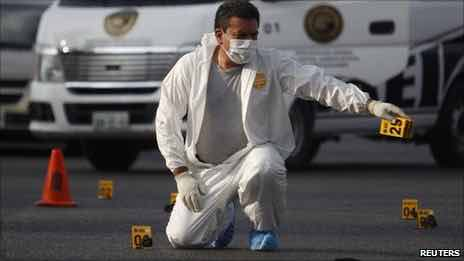
\includegraphics[scale=.48]{pics/csi-team}
  \end{center}
  \item 首要任務: priority, primary responsibility
  \item 裝修: renovation / refurbishment
  \item 破案: clear up / break / solve the case
\end{itemize}
\end{multicols}

\subsubsection*{需要掌握的句型}
\begin{multicols}{2}
\begin{itemize}
  \itemsep0em
  \item 另外兩個中的其中一個: one of the other two
  \item 這前後只有五分鐘: It all happened within 5 mins.
  \item 價值***的香煙: cigarettes \hilight{valued at} ***.
  \item 我從來沒想到這會發生在我身上: I didn't expect it would happen to me.
  \item 難道你們的首要任務不是保護市民的財產和安全嗎: Isn't protecting the property \& safety of the residents your primary responsibility? 
\end{itemize}
\end{multicols}

\subsection{商店盜竊}
\subsubsection*{需要掌握的單詞短語}
\begin{multicols}{2}
\begin{itemize}
  \itemsep0em
  \item 燭台: candle holder
  \item 尿布: nappy / diaper
  \item 嬰兒車: pram
  \item 公訴人: public prosecutor
  \item 監控錄像: security \hilight{footage}
  \begin{center}
    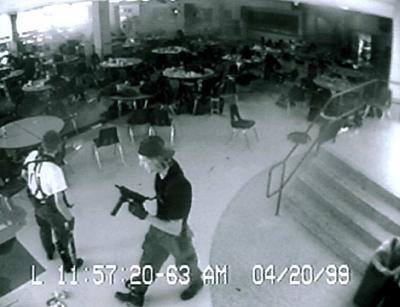
\includegraphics[scale=.55]{pics/security-footage}
  \end{center}
  \item 貨架: rack
  \item 兩個中的另外一個: the other
  \item 檢查(包): \hilight{inspect}, check
  \item 否認, 不配合(的態度): denial
  \item 人格擔保: character reference
  \item \hilight{誠實}: integrity
  \item 書面的證明證詞: testimony
\end{itemize}
\end{multicols}

\subsubsection*{需要掌握的句型}
\begin{multicols}{2}
\begin{itemize}
  \itemsep0em
  \item 移交給某人: pass $sth.$ to / onto $sb.$
  \item 被指控: be charged with...
  \item 他們冤枉我了: \hilight{They wronged me}.
  \item 看了錄像: have accessed to the security footage.
  \item 某事說不通: $sth.$ does not make sense.
  \item 證明某人的清白: prove my innocence
\end{itemize}
\end{multicols}

\vspace{15mm}

\begin{center}
  \textbf{************ END OF THE DAY ************}
\end{center}
\newpage

\section{2016年2月23日 (Instructor: Chris)}
\subsection{男朋友移民咨詢}
\mybox{\centering \textbf{注意}: 更多內容請見詞彙專題里的和澳洲移民相關簽證!}
\subsubsection*{需要掌握的單詞短語}
\begin{multicols}{2}
\begin{itemize}
  \itemsep0em
  \item 技術職業列表: Skilled Occupational List
  \item 職業評估: \hilight{Skill Assessment}
  \item 家庭團聚: family reunion
  \item 偏遠地區: \hilight{regional} area
  \item 雇主擔保: employer's sponsor
  \item 移民傾向: \hilight{tendency to migrate}
  \item 傾向, 目的: tendency / \hilight{inclination} / intention
  \item 間隔年: gap year\footnote{a gap year is a year before going to college or University and after finishing high school or taking a year off before going into graduate school after completing a bachelor as an undergraduate.}
  \item 事實婚姻關係: de facto relationship
\end{itemize}
\end{multicols}

\subsubsection*{需要掌握的句型}
\begin{multicols}{2}
\begin{itemize}
  \itemsep0em
  \item 讓我們回憶一下: \hilight{I take you back to + 日期}
  \item 徹底忘乾淨: throw $sth.$ out of the window
  \item 我怎麼會忘呢: How could I forget?
\end{itemize}
\end{multicols}

\subsubsection*{注意}
\begin{itemize}
  \itemsep0em
  \item Permanent Residency 一般代表政府發放的簽證, Permanent Residency 一般代表移民的狀態, 而Permanent Resident 只能指代拿到簽證的人.
  \item 可以瞭解一下澳洲常見簽證對應的編號, 這樣可以加速筆記, 具體可以參考話外音里的``澳大利亞簽證及其編號"!
\end{itemize}

\subsection{法庭交互式盤問}
\subsubsection*{需要掌握的單詞短語}
\begin{multicols}{2}
\begin{itemize}
  \itemsep0em
  \item 公平交易庭: Fair Trading
  \item 新州民事與行政仲裁庭: NCAT (NSW Civil and Administrative Tribunal)
  \item Fair Trading $\xrightarrow{\text{如果解決不了}}$ NCAT
  \item 調解: \hilight{conciliation / mediation}
  \item 調解員: conciliator / mediator
  \item 仲裁庭的仲裁員 / 仲裁官: member
  \item 攔下來: apprehend
  \item 嚇傻了: dumb-founded
  \item 文具: stationary
  \item 在特價 / 在打折: \hilight{on special} / discount
  \item 同等價值優惠券: rain check\footnote{原意: a ticket given for later use when a sporting fixture or other outdoor event is interrupted or postponed by rain.}
  \item 禮品註冊處(婚禮): gift registry
  \begin{center}
    
\includegraphics[scale=.4]{pics/gift-registry}
  \end{center}
  \item 專門放紅包的地方 (婚禮): wish well (也可以指許願池)
  \item 心不在焉, 腦子不在這: absent-minded
  \item \hilight{還}款付清: pay off
  \item 監控攝像頭: surveillance camera
  \item 監控錄像: surveillance footage
  \item (從被告席上)下來: stand down
  \item 有 / 無宗教信仰宣誓: oath\footnote{An oath is a verbal promise to tell the truth. Oaths are frequently made while holding the Bible, the New Testament or the Old Testament.} / affirmation\footnote{An affirmation is a verbal, solemn and formal declaration, which is made in place of an oath.}
\end{itemize}
\end{multicols}

\subsubsection*{需要掌握的句型}
\begin{multicols}{2}
\begin{itemize}
  \itemsep0em
  \item 讓我們回憶一下: I take you back to + 日期
  \item 徹底忘乾淨: throw $sth.$ out of the window
  \item 我怎麼會忘呢: How could I forget?
  \item 把商品臨時預定下來: put $sth.$ on layby
  \item 下次再去(表謝絕): take a raincheck?
  \item 過期不候: no rain check!
  \item 我這麼跟你說吧: I put it to you that...\footnote{言外之意: 我不信你所說的那些bullshit}
  \item 難道我被羞辱的還不夠嗎: Haven't I been humiliated more than enough?
  \item 讓某人出庭作證: put $sb.$ on the stand
  \item (法庭)我可以走了嗎: Can I be excused?
  \item (法庭)你可以走了: You can be excused.
\end{itemize}
\end{multicols}

\subsubsection*{注意}
\begin{itemize}
  \itemsep0em
  \item Don't you think 和 What if 後面要接陳述句!
\end{itemize}

\subsection{移民上訴仲裁庭}
\subsubsection*{需要掌握的單詞短語}
\begin{multicols}{2}
\begin{itemize}
  \itemsep0em
  \item 濕疹\footnote{濕疹是一種常見的過敏性皮膚病. 濕疹一詞通常泛指一系列持久和續發的皮疹, 以發紅, 水腫, 瘙癢和發乾為表徵, 可伴有結痂, 剝落, 起泡, 開裂, 出血或滲血.}: eczema
  \item 麻疹 / 蕁麻疹\footnote{蕁麻疹俗稱風團或風疹塊, 有的地區叫鬼風疙瘩, 中醫稱癮疹, 客語稱冷瘼, 是一種皮膚過敏. 症狀是局部皮膚忽然成塊地紅腫, 發癢, 幾小時後消退, 不留痕跡.} : measles / hives
  \item 風疹: German measles
  \item 不吃早飯: skip the breakfast
  \item 萬能的主: mighty god
  \item 有法律效力的, 有約束力的: binding
  \item 悶悶不樂: blue
  \item 不清醒的: \hilight{disoriented} / not clear-minded
\end{itemize}
\end{multicols}

\subsubsection*{需要掌握的句型}
\begin{multicols}{2}
\begin{itemize}
  \itemsep0em
  \item 是否還在: ... still there
\end{itemize}
\end{multicols}

\subsection{律師對話 - 家庭暴力禁止令}
\subsubsection*{需要掌握的單詞短語}
\begin{multicols}{2}
\begin{itemize}
  \itemsep0em
  \item 反社會人格: sociopath
  \item 沙包: punch bag
  \item (房門口的)腳墊: door mat
  \item 攻擊: assault
  \begin{center}
    
\includegraphics[scale=.6]{pics/assault}
  \end{center}
  \item 發洩: vent
  \item 酒醉鬼: alcoholic
  \begin{center}
    
\includegraphics[scale=.35]{pics/alcoholic}
  \end{center}
  \item 出路: \hilight{the way out}
  \item 八卦 / 謠傳: \hilight{gossip} / rumour
  \item 贍養費: maintenance
  \item 放棄: forgo
  \item 應得的財產: fair share
  \item 爭: fight over
  \item 眼鏡: spectacle
  \item 每天的折磨: \hilight{daily} torture
  \item 臨時判決書: decree nisi
  \item 最終判決書: decree absolute
  \item 達成和解: reach a reconciliation
\end{itemize}
\end{multicols}

\subsubsection*{需要掌握的句型}
\begin{multicols}{2}
\begin{itemize}
  \itemsep0em
  \item 與某人相處: get along with ...
  \item 喝醉酒回家: \hilight{come home drunk}
  \item (輕)打屁股: spank the bottom
  \item 忍受: \hilight{put up with...}
  \item 進而看下一步: take it from there.
  \item 出洋相: to make a spectacle of oneself
  \item 把某人當出氣筒: \hilight{treat $sb.$ as punch bag / door mat}
  \item 拿某人出氣: \hilight{vent} / take it out on $sb.$
\end{itemize}
\end{multicols}

\subsection{法律咨詢 - 家庭暴力禁止令}
\subsubsection*{需要掌握的單詞短語}
\begin{multicols}{2}
\begin{itemize}
  \itemsep0em
  \item 過錯離婚: no-fault divorce
  \item 工作人員: support officer
  \item 列出: set out = list
  \item 暴怒: furious (with $sb.$)
  \item 違反(法律): breach
  \item 淤青: bruise
  \item 發紅: redness
  \item 血痕: blood stain
  \item 疤 / 痂: scar / scab
  \item 青一塊紫一塊: black and blue
\end{itemize}
\end{multicols}

\subsubsection*{需要掌握的句型}
\begin{multicols}{2}
\begin{itemize}
  \itemsep0em
  \item 渾然不知, 不知所措: be confused and at a loss.
  \item 關在監獄: be locked up in jail / gaol
  \item 在中國沒有這回事: there is no such thing in China.
  \item 求助於某人: turn to $sb.$ (for help)
\end{itemize}
\end{multicols}

\subsection{家庭暴力 - 干涉令}
\subsubsection*{需要掌握的單詞短語}
\begin{multicols}{2}
\begin{itemize}
  \itemsep0em
  \item 報復: revenge / get back \hilight{at}
  \item (法律文件)起效力: in force
  \item 安全感: sense of security
  \item 遵紀守法: law-abiding
\end{itemize}
\end{multicols}

\subsubsection*{需要掌握的句型}
\begin{multicols}{2}
\begin{itemize}
  \itemsep0em
  \item 送達: be served on...
\end{itemize}
\end{multicols}

\vspace{15mm}

\begin{center}
  \textbf{************ END OF THE DAY ************}
\end{center}
\newpage